% \begin{figure}
\begin{tabular}{@{}c@{}c@{}}
\begin{subfigure}[b]{0.5\textwidth}
\begin{center}
{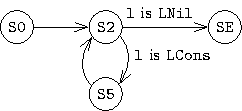
\includegraphics[scale=1.4]{chapters/figures/figSumListSpecCfg.pdf}}
\end{center}
\caption{\label{fig:llTraverseSpecCFG}CFG of \SpecL{} procedure}
\end{subfigure}%
&
\begin{subfigure}[b]{0.5\textwidth}
\begin{center}
{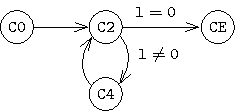
\includegraphics[scale=1.4]{chapters/figures/figSumListCCfg.pdf}}
\end{center}
\caption{\label{fig:llTraverseCCFG}CFG of C procedure}
\end{subfigure}%
\\
\end{tabular}
\caption{\label{fig:llTraverseSpecAndCCFG}CFG representation of \SpecL{} and C IRs in \cref{fig:llTraverseSpecIR,fig:llTraverseCIR} for the {\tt sum\_list} procedures in \cref{fig:llTraverseSpec,fig:llTraverseC} respectively.}
\end{figure}
